\documentclass{article}

% if you need to pass options to natbib, use, e.g.:
% \PassOptionsToPackage{numbers, compress}{natbib}
% before loading nips_2016
%
% to avoid loading the natbib package, add option nonatbib:
% \usepackage[nonatbib]{nips_2016}

\usepackage[final]{nips_2016}
\usepackage{soul}
\usepackage{xcolor}

% to compile a camera-ready version, add the [final] option, e.g.:
% \usepackage[final]{nips_2016}

\usepackage[utf8]{inputenc} % allow utf-8 input
\usepackage[T1]{fontenc}    % use 8-bit T1 fonts
\usepackage{hyperref}       % hyperlinks
\usepackage{url}            % simple URL typesetting
\usepackage{booktabs}       % professional-quality tables
\usepackage{amsfonts}       % blackboard math symbols
\usepackage{nicefrac}       % compact symbols for 1/2, etc.
\usepackage{microtype}      % microtypography
\usepackage{numprint}
\usepackage[english]{babel}
\usepackage{graphicx}

\title{MorphoDeep: deep learning for Hungarian morphology\\MorphoDeep: deep learning magyar morfol\'ogi\'ara}

% The \author macro works with any number of authors. There are two
% commands used to separate the names and addresses of multiple
% authors: \And and \AND.
%
% Using \And between authors leaves it to LaTeX to determine where to
% break the lines. Using \AND forces a line break at that point. So,
% if LaTeX puts 3 of 4 authors names on the first line, and the last
% on the second line, try using \AND instead of \And before the third
% author name.

\author{
  Judit \'Acs\thanks{http://avalon.aut.bme.hu/~judit} \\
  Department of Automation and Applied Informatics \\
  Budapest University of Technology and Economics\\
  \texttt{judit@aut.bme.hu} \\
}

\begin{document}

\maketitle

\begin{abstract}
    We present three types of experiments pertaining to Hungarian morphology.
    The first type is the classification of part-of-speech tags, the second type is the classification of frequent inflectional paradigms.
    Lastly, we use clusters of morphological tags as classes.
    All of our experiments apply feed forward neural networks and recurrent neural networks.
    Our data is the Hungarian Webcorpus including morphological analysis by a rule-based analyzer.

    Ebben a munkában háromféle, magyar morfológiai jelenségeket vizsgáló kísérletek eredményeit mutatjuk be.
    Az első típus a szófaji címkék osztályozása, a második néhány gyakori ragozás vizsgálata, míg a harmadik a morfológiai elemzések előzetes klaszterezése utáni osztályozás.
    Mindegyik kísérlethez előrecsatolt, illetve rekurrens neurális hálókat alkalmazunk.
    A kísérletek adatait a Magyar Webcorpus morfológiailag elemzett változata szolgáltatja.
\end{abstract}

\section{Introduction}\label{sec:introduction}

Morphology is the study of word structure, how words are formed and how they are related to each other.
Traditionally linguists define \emph{morpheme} as the smallest unit that has semantic meaning on its own.
Morphological analysis is the process of segmenting words into smaller units, called \emph{morphemes} and analysing their syntactic and semantic roles.

Morphemes are either \emph{bound} or \emph{free}.
Bound morphemes may only appear as parts of a larger word, while free or unbound morphemes stand on their own.

Bound morphemes are further categorized into \emph{derivational} and \emph{inflectional} morphemes.
The former category consist of morphemes that change the grammatical category or the meaning of the word, while the latter category only affects plurality, tense, case and so on.

Morphological analysis plays a central role in many natural language processing tasks such as information retrieval, machine translation or spell checking.
However, the large variation of morphological paradigms accross different languages makes it especially hard to create general solutions for morphological analysis.
For example Chinese or Vietnamese are both \emph{isolating languages} i.e.~they almost exclusively use free morphemes, therefore analysis below word level is seldom hard or necessary.
In contrast, Uralic languages such as Hungarian exhibit rich morphology, and the number of unique word forms is basically infinite.
English -- by far the most well resourced language -- lies somewhere in the middle, therefore most general solutions do not focus as much on morphology as for example Hungarian NLP would necessitate.

In this work, we shall only examine bound morphemes and mostly inflectional paradigms based on word forms in Hungarian.


\section{Related work}\label{sec:related}

Morphology is one of the last areas of natural language processing, where rule based systems still heavily outperform machine learning systems.
Particularly, the unsupervised learning of morphology is very hard to perform.
Perhaps the most significant attempt at unsupervised segmentation and basic analysis is \emph{Morfessor} \cite{Creutz:2002, Creutz:2007}.
Morfessor uses Hidden Markov Models to model simple morphology (prefix-stem-suffix).

\cite{Goldsmith:2001} and \cite{Hammarstrom:2011} give an overview of the unsupervised learning of morphology before the era of deep learning.

Morphology has been receiving a lot more attention from the deep learning community and this year a shared task was organized by SIGMORPHON'16. \cite{Cotterell:2016}
The task was morphological reinflection in a high number of languages including Hungarian.
The top performers all used deep learning, the best one \citep{Kann:2016} outperforming others with a 10\% margin in certain languages.

Other recent papers on the supervised learning of morphological paradigms include \cite{Durrett:2013} and \cite{Ahlberg:2015}.

\section{Classification problems}\label{sec:classification}

Our experiments can be grouped into three categories.
All experiments use a single word and its analysis as a sample, no context is taken into account.
Our training data is the Hungarian Webcorpus \cite{Halacsy:2004}, which includes morphological analysis by HunMorph \cite{Tron:2005}.
We consider the output of HunMorph -- a rule-based analyzer -- to be very reliable and treat the data as a high quality silver standard.
Character n-grams were extracted as features.

\subsection{Classifying part-of-speech tags}

\emph{Part of speech} is a category of words that display similar grammatical properties.
The assignment of part of speech categories to words is called \emph{part of speech tagging} or {POS tagging}.
POS tagging is usually a crucial task in NLP and high quality tools are necessary.
We investigate how well POS tags can be inferred from word forms using the output of HunMorph which includes POS tags.
POS tagging can be considered as a baseline task of morphological analysis, since high quality morphological analysis includes and extends high quality POS tagging.

The number of different POS tags is very limited, only 10 categories take up at least 1\% of the words (see Table~\ref{table:pos-tags}).

\begin{table}[t]
  \caption{Frequency of the top 10 POS tags in 1 million words}
  \label{table:pos-tags}
  \centering
  \begin{tabular}{cc}
      \toprule
      POS & Frequency \\
      \midrule
      NOUN & 311259 \\
      PUNCT & 162867 \\
      VERB & 105032 \\
      ART & 100766 \\
      ADJ & 85076 \\
      ADV & 67105 \\
      CONJ & 55539 \\
      NUM & 19446 \\
      POSTP & 16480 \\
      PREV & 12691 \\
      \bottomrule
  \end{tabular}
\end{table}

Since punctuation (\texttt{PUNCT}) and article (\texttt{ART}) are \emph{closed} categories -- i.e.~their members can be easily listed and the list is not very long --, they do not amount to an interesting classification problem and most of our experiements aim to distinguish between nouns and verbs.
In Hungarian this is an almost trivial task for any competent speaker and we expect a learning algorithm to perform well too.

\subsection{Inflectional paradigm classification}

In Hungarian syntactic and semantic roles of words are most frequently marked with suffixes.
Inferring inflectional paradigms from word forms without context is also an easy task for a human and should be easy for a learning algorithm too.
We chose a few frequent inflectional paradigms for classification:

\begin{description}
    \item[singular vs.~plural] both verbs and nouns can be singular and plural and we make no distinction between verbs and nouns in this case,
    \item[first person vs.~second person] whether a verb is first or second person (conjugation),
    \item[accusative vs.~other noun cases] among the dozens of noun cases, accusative is the most common,
    \item[past tense vs.~present tense] verb tenses regardless of the person,
    \item[conditional verbs vs.~others] verbs in conditional or other case,
    \item[most frequent noun cases] 10 most frequent noun cases.
\end{description}

\subsection{Classification of tag clusters}

Full morphological analysis is represented via a complicated coding, called \emph{KR coding}, which contains among others POS, case, tense and plurality.
The number of unique tags in the first million words is about \numprint{1700}.
The large number of different tags call for some kind of aggregation such as clustering.

Brown clustering is a hierarchical clustering method that uses a mutual information criteria for merging two clusters.
As a hierarchical clustering method, Brown clustering eventually results in one big cluster unless a stopping criteria is specified.
For our experiments we limit the number of clusters to 120.
It is important to note that only the tags are used during clustering and word forms are ignored.

\section{Feature extraction}

The corpus contains a single word and its analysis per line and sentence boundaries are denoted with an empty line.
Words and KR codes are tab separated.
Since the corpus is already denoised and tokenized, the only preprocessing we use is lowercasing.

Our assumption is that the end of the word is more implicative of its grammatical category than its beginning, due to the agglutinative (rich in suffixes) nature of Hungarian.
Character n-grams are used as features starting from the end of the word.
The position of the n-grams are also preserved (i.e.~this is not a bag-of-ngrams model).
Table~\ref{table:feat_extract} shows an example of feature extraction.

\begin{table}[t]
    \caption{Bigram features using the last 6 characters. The sample word is \emph{nevetés}.}
  \label{table:feat_extract}
  \centering
  \begin{tabular}{cc}
      \toprule
      Feature (start index) & Value \\
      \midrule
      -1 & é\$ \\
      -2 & és \\
      -3 & té \\
      -4 & et \\
      -5 & ve \\
      -6 & ev \\
      \bottomrule
  \end{tabular}
\end{table}

Padding characters are added to the beginning of the words if they are shorter than the number of features extracted.
The last character of the word is usually especially important, therefore $N-1$ padding characters are added to the end of the word.
When using recursive neural networks, we exclude position information.

\section{Experimental setup}

Each experiment involves 4 steps:

\begin{enumerate}
    \item feature extraction: Webcorpus is read from the beginning until enough samples are collected,
    \item training: train on 90\% of the samples (split into 80\% train and 20\% validation set),
    \item testing: test on 10\% of the samples,
    \item logging: save the experiment to a pandas DataFrame.
\end{enumerate}

\subsection{Architecture}

The first architecture tested was a simple feed forward neural network.
Since the length of the input is limited to 5-10 characters, we limit the depth of the network to two hidden layers (to be fair, three hidden layers were found not to improve the results while significantly increase training time), and the number of neurons-per-layer to 100.
Grid search like optimization is performed in these boundaries.

Secondly recurrent neural networks were used with varying number of cells.

\subsection{Technical background}

For training and testing neural networks we use Keras with Tensorflow backend.
FFNN experiments were run in a Jupyter notebook, while RNN experiments were implemented as standalone scripts.
The reason for this is that the codebase is under heavy development and constant refactoring with the eventual goal of creating an experiment framework as a Python package.

Every experiment is logged into a pandas DataFrame and saved to disk in a tab-separated file.
FFNN and RNN experiments log into separate DataFrames and both files are versioned.
Each line represents a single experiment with all its parameters and results.
Due to the large number of parameters, the tables are not easy on the human eyes, and a human readable version with fewer lines is also extracted and saved.
GitHub natively renders tsv as tables.

\section{Parameter optimization and results}

Feature extraction involves several parameters:

\begin{description}
    \item[last\_char] the number of characters starting from the end of the word, to be used as features,
    \item[N] the size of n-grams etracted,
    \item[include\_smaller\_ngrams] include $1\dots N$ grams in the features,
    \item[use\_padding] use padding characters at the beginning and the end of words,
    \item[sample\_per\_class] how many samples-per-class are to be extracted.
\end{description}

Setting \texttt{include\_smaller\_ngrams} and \texttt{use\_padding} \texttt{True} were found to help during the first half of the experiments and for the sake of simplicity were kept that way later on.
The number of training samples is only limited by the available GPU memory.
\numprint{60000} samples split into 90\% train and 10\% test can be easily trained on our system.
We did experiment with more samples, but the gain in accuracy was not substantial.
Although there are ways to avoid loading everything into memory, we have not experimented with them yet.

Model hyperparameters include the number of hidden layers, the number of neurons in the hidden layers, the number LSTM and GRU cells, the learning rate and the optimizer's parameters such as the loss function.
Training parameters include the number of epochs and the batch size.
The training data was split into 80\% training and 20\% validation and early stopping was performed using the latter.
Each layer applied sigmoid activation function.

\subsection{POS classification}

Most of our experiments were run on noun vs.~verb, so we shall go into detail regarding this case.

\subsubsection{NOUN vs.~VERB classification}

The highest test accuracy we achieved using a feed forward network, was 96.73\% using trigram features from the last 10 characters.

Since recurrent neural networks are able to ''memorize'' previous inputs, we can feed the samples as sequences of characters and expect the network to infer n-gram like features.
We experiment with LSTM and GRU and the 95.61\% using GRU with 125 cells and limiting the input sequence to the last 9 characters.
Although the best configuration was achieved using GRU, it is not at all clear whether LSTM or GRU are better suited for this task.
Figure~\ref{fig:lstm_gru} demonstrates the very small difference between the results and other comparisons are available in the repository.

\begin{figure}[h]
    \centering
    \label{fig:lstm_gru}
    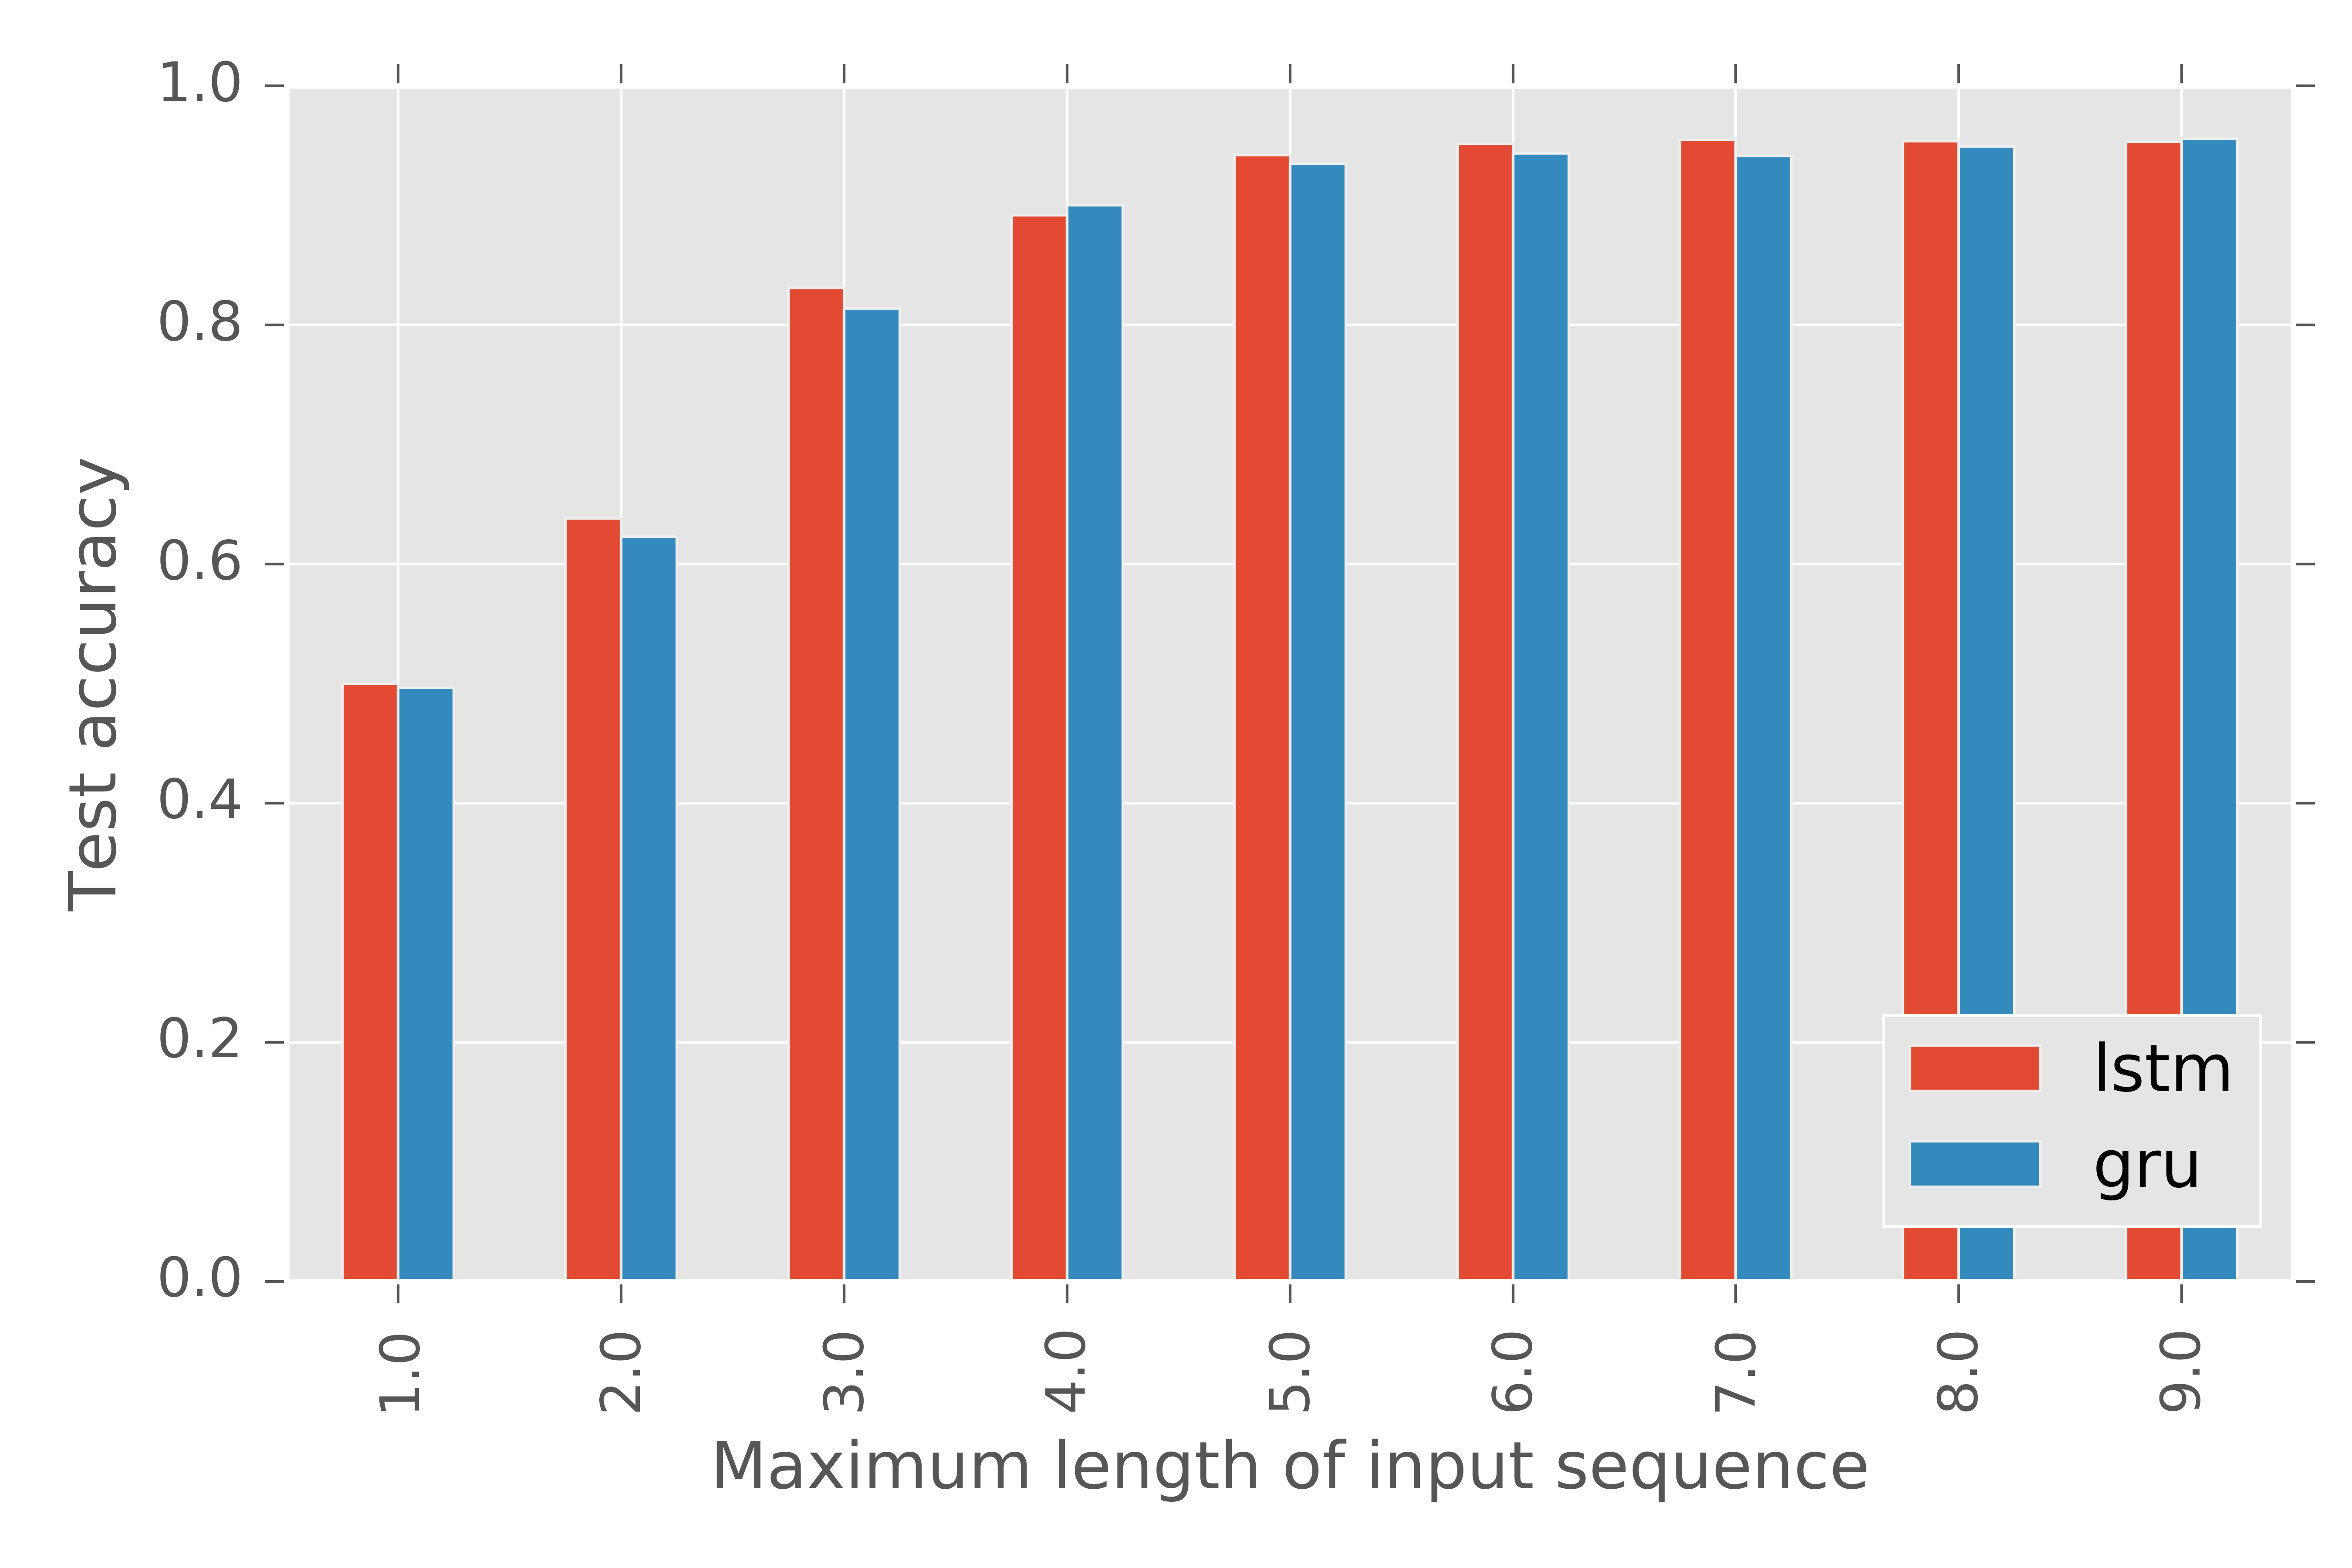
\includegraphics[width=\textwidth]{lstm_gru}
      \caption{LSTM vs.~GRU against varying sequence length}
\end{figure}

\subsubsection{Other part-of-speech categories}

A few experiments were run on other category combinations, see Table~\ref{table:other_pos} for the results.
\begin{table}[t]
    \caption{Highest test accuracy for inflectional paradigms.}
    \label{table:other_pos}
    \centering
    \begin{tabular}{ccc}
        \toprule
        POS & FFNN & RNN \\
        \midrule
        adverb, adjective & 97.6 & 96.8 \\
        conjunction, noun & 99.1 & 98.3 \\
        adjective, conj, noun, verb & 85 & 87.43 \\
        \bottomrule
    \end{tabular}
\end{table}



\subsection{Inflectional paradigms}

We run the same experiments on a selected few paradigms that occur frequently in Hungarian.
The results are listed in Table~\ref{table:inf_paradigms}.

\begin{table}[t]
    \caption{Highest test accuracy for inflectional paradigms.}
    \label{table:inf_paradigms}
    \centering
    \begin{tabular}{ccc}
        \toprule
        Paradigm & FFNN & RNN \\
        \midrule
        singular/plural & 99.7 & 99\\
        first/second person & 98.9 & 99.6 \\
        accusative/non-accusative & 99.8 & 99.6\\
        past tense/present tense & 99.4 & 98.1 \\
        conditional verbs & 99.9 & 100 \\
        10 noun cases & 99.3 & 99.3 \\
        \bottomrule
    \end{tabular}
\end{table}

\subsection{Classifying tag clusters}

The significance of this experiment group is twofold: (i) the number of classes is considerably higher than previously, (ii) the clusters were created with no regard to word forms.
If a word-based classifier is able to learn these clusters, the clustering does convey some kind of word information.

For these experiments we need additional preprocessing, namely we have to convert KR codes to cluster ids using an already existing mapping.
The distribution of tags in a cluster is very far from uniform, with a few tags dominating each class.
To avoid learning single tags instead of clusters, we limit the number of times a tag (mapped to a cluster id) may appear in the training data.

By limiting the number of tags-per-cluster to 25 and requiring 100 samples, the classifier is able to achive close to 60\% accuracy.
When we do not limit the tags-per-cluster, accuracy reaches 70\% on 120 classes.

\section{Conclusion and future work}

Our experiments show that all three tasks are relatively easy to solve with simple neural network architectures and a modest number of hidden layers and neurons.
While FFNN are very simple, the obvious advantage of RNN is that raw character features can be fed to the network instead of fiddling with n-grams.
One of the next steps would be to interpret the features learned by the network.

The eventual goal of this research project is the unsupervised discovery of morphological paradigms.
Our study suggests that once these paradigms are labeled, it is very easy to distinguish them from each other.
However, the biggest obstacle is the large number of paradigms and their uneven distribution, which makes the data very sparse.

Although we do have high quaility rule-based analyzers for Hungarian, this is not true for many other languages.
A possible application of this line of research would be to extend it to other languages such as low-density Uralic languages with rich morphology.

For the machine learning background, only very simple approaches were compared since the task itself did not necessitate more sophisticated solutions.
We do plan to apply other neural network architectures later on for automatic segmentation and rule discovery.

\begin{thebibliography}{10}

\bibitem{Ahlberg:2015}
Malin Ahlberg, Markus Forsberg, and Mans Hulden.
\newblock Paradigm classification in supervised learning of morphology.
\newblock In {\em Proc. of NAACL}, 2015.

\bibitem{Cotterell:2016}
Ryan Cotterell, Christo Kirov, John Sylak-Glassman, David Yarowsky, Jason
  Eisner, and Mans Hulden.
\newblock The sigmorphon 2016 shared task---morphological reinflection.
\newblock In {\em Proceedings of the 2016 Meeting of SIGMORPHON}, Berlin,
  Germany, August 2016. Association for Computational Linguistics.

\bibitem{Creutz:2002}
Mathias Creutz and Krista Lagus.
\newblock Unsupervised discovery of morphemes.
\newblock In {\em Proc. 6th SIGPHON}, pages 21--–30, 2002.

\bibitem{Creutz:2007}
Mathias Creutz and Krista Lagus.
\newblock Unsupervised models for morpheme segmentation and morphology
  learning.
\newblock {\em ACM Transactions on Speech and Language Processing (TSLP)},
  4(1):3, 2007.

\bibitem{Durrett:2013}
Greg Durrett and John DeNero.
\newblock Supervised learning of complete morphological paradigms.
\newblock 2013.

\bibitem{Goldsmith:2001}
John~A. Goldsmith.
\newblock Unsupervised learning of the morphology of a natural language.
\newblock {\em Computational Linguistics}, 27(2):153--198, 2001.

\bibitem{Halacsy:2004}
P\'eter Hal\'acsy, Andr\'as Kornai, L\'aszl\'o N\'emeth, Andr\'as Rung,
  Istv\'an Szakad\'at, and Viktor Tr\'on.
\newblock Creating open language resources for {H}ungarian.
\newblock In {\em {Proceedings of the Fourth International Conference on
  Language Resources and Evaluation (LREC 2004)}}, pages 203--210. ELRA, 2004.

\bibitem{Hammarstrom:2011}
Harald Hammarstr{\"o}m and Lars Borin.
\newblock Unsupervised learning of morphology.
\newblock {\em Computational Linguistics}, 37(2):309--350, 2011.

\bibitem{Kann:2016}
Katharina Kann and Hinrich Sch{\"u}tze.
\newblock Med: The lmu system for the sigmorphon 2016 shared task on
  morphological reinflection.
\newblock {\em ACL 2016}, page~62, 2016.

\bibitem{Tron:2005}
Viktor Tr{\'o}n, Gy\"{o}gy Gyepesi, P\'{e}ter Hal\'{a}csky, Andr\'{a}s Kornai,
  L\'{a}szl\'{o} N\'{e}meth, and D\'{a}niel Varga.
\newblock Hunmorph: Open source word analysis.
\newblock In {\em {Proceedings of the ACL Workshop on Software}}, pages 77--85.
  Association for Computational Linguistics, Ann Arbor, Michigan, 2005.

\end{thebibliography}
\end{document}

